\documentclass{scrreprt}

\usepackage{aligned-overset}
\usepackage{amsmath}
\usepackage{amsthm}
\usepackage{amssymb}
\usepackage{bm}
\usepackage[inline, shortlabels]{enumitem}
\usepackage{hyperref}
\usepackage[utf8]{inputenc}
\usepackage{listings}
\usepackage{multicol}
\usepackage{mathtools}
\usepackage{pdflscape}
\usepackage{physics}
\usepackage{polynom}
\usepackage{tabularx}
\usepackage[table]{xcolor}
\usepackage{titling}
\usepackage{fancyhdr}
\usepackage{xfrac}
\usepackage{pgfplots}

\pgfplotsset{compat = newest}
\usepgfplotslibrary{fillbetween}
\usetikzlibrary{arrows, arrows.meta}
\usetikzlibrary{calc}
\usetikzlibrary{patterns}

\author{Karsten Lehmann}
\date{WiSe 2024/25}
\title{Übungsblatt 13\\INF-B-110, Diskrete Strukturen}

\setlength{\parindent}{0pt}

\setlength{\headheight}{26pt}
\pagestyle{fancy}
\fancyhf{}
\lhead{\thetitle}
\rhead{\theauthor}
\lfoot{\thedate}
\rfoot{Seite \thepage}

\newcommand{\ggT}[0]{\text{ggT}}
\DeclarePairedDelimiter{\floor}{\lfloor}{\rfloor}

\begin{document}
\paragraph{Ü 13.1}

Ermitteln Sie für jeden Baum aus Aufgabe 9.3, wie viele Bäume mit Knotenmenge
$V = \qty\big{1, \ldots, 5}$ zu ihm isomorph sind.

Überprüfen Sie Ihr Ergebnis, indem Sie die Gesamtzahl aller möglichen Bäume mit
Knotenmenge $V$ mit Hilfe des Satzes von Cayley berechnen.

\subparagraph{Lsg.} Es war Aufgabe 9.3 (a): \emph{``Geben Sie bis auf Isomorphie
  alle möglichen Diagramme von Bäumen $T = \qty\big(V, E)$ an, für die
  $\abs{V} + \abs{E} = 9$ gilt''} und die Lösung dazu war

\begin{minipage}{.2\textwidth}
  \begin{tikzpicture}
    \foreach \y in {0,...,4} {
      \node[circle, draw, inner sep=0pt, minimum size=1mm] (\y) at ($(0,{\y/3})$) {};
    }

    \draw (0) -- (1) -- (2) -- (3) -- (4);

    \node at (0, -0.5) {$G_1$};
  \end{tikzpicture}
\end{minipage}
\begin{minipage}{.2\textwidth}
  \begin{tikzpicture}
    \foreach \y in {0,...,3} {
      \node[circle, draw, inner sep=0pt, minimum size=1mm] (\y) at ($(0,{\y/2})$) {};
    }
    \node[circle, draw, inner sep=0pt, minimum size=1mm] (4) at (0.5,1) {};
    \draw (0) -- (1) -- (2) -- (3);
    \draw (2) -- (4);

    \node at (0, -0.5) {$G_2$};
  \end{tikzpicture}
\end{minipage}
\begin{minipage}{.2\textwidth}
  \begin{tikzpicture}
    \foreach \y in {0,...,2} {
      \node[circle, draw, inner sep=0pt, minimum size=1mm] (\y) at ($(0,{\y/2})$) {};
    }
    \node[circle, draw, inner sep=0pt, minimum size=1mm] (3) at (0.5,0.5) {};
    \node[circle, draw, inner sep=0pt, minimum size=1mm] (4) at (-0.5,0.5) {};
    \draw (0) -- (1) -- (2);
    \draw (1) -- (3);
    \draw (1) -- (4);

    \node at (0, -1) {$G_3$};
  \end{tikzpicture}
\end{minipage}

Meine Überlegung ist, für jeden der Graphen zu schauen, welche Punkte ich
minimal fixieren muss, um Isomorphismen eindeutig zu bestimmen.
\begin{itemize}
\item[$G_3$:] Die Isomorphismen des Graphen sind durch den Knoten in der Mitte
  eindeutig bestimmt.

  $\Rightarrow 5$ Isomorphismen

\item[$G_2$:] Die Isomorphismen sind eindeutig bestimmt, durch die Kombination
  aus
  \begin{enumerate}[(1)]
  \item dem Knoten von Grad 3
  \item dem Knoten vom Grad 2
  \item dem Blatt am Knoten von Grad 2
  \end{enumerate}

  $\Rightarrow 5 \cdot 4 \cdot 3 = 60$ Isomorphismen

\item[$G_1$:] Die Isomorphismen sind eindeutig bestimmt, durch die Kombination
  aus
  \begin{enumerate}[(1)]
  \item dem Knoten in der Mitte
  \item die beiden Blätter ohne Reihenfolge, $\binom{4}{2} = 6$
  \item der Knoten am kleineren der Beiden Blätter
  \end{enumerate}

  $\Rightarrow 5 \cdot 6 \cdot 2 = 60$ Isomorphismen
\end{itemize}

Schließlich ist nach dem Satz von Cayley, \emph{``Für alle
  $n \in \mathbb{N} \setminus \qty\big{0}$ gilt $t\qty\big(n) = n^{n - 2}$''}
die Anzahl aller Bäume mit 5 Knoten $t\qty\big(5) = 5^3 = 125$.

\newpage
\paragraph{Ü 13.2}
\begin{enumerate}[(a)]
\item Bestimmen Sie den Prüfercode folgender Bäume

  \begin{minipage}{.45\textwidth}
    \begin{tikzpicture}
      \node[circle, draw, inner sep=0pt, minimum size=1mm, label=above right:{$0$}] (0) at (0,0) {};
      \node[circle, draw, inner sep=0pt, minimum size=1mm, label=above:{$1$}] (1) at (1,0) {};
      \node[circle, draw, inner sep=0pt, minimum size=1mm, label=above left:{$2$}] (2) at (2,0) {};
      \node[circle, draw, inner sep=0pt, minimum size=1mm, label=above right:{$3$}] (3) at (2.5,1) {};
      \node[circle, draw, inner sep=0pt, minimum size=1mm, label=left:{$4$}] (4) at (-1,0) {};
      \node[circle, draw, inner sep=0pt, minimum size=1mm, label=above left:{$5$}] (5) at (-0.5,1) {};
      \node[circle, draw, inner sep=0pt, minimum size=1mm, label=below left:{$6$}] (6) at (-0.5,-1) {};
      \node[circle, draw, inner sep=0pt, minimum size=1mm, label=below:{$7$}] (7) at (1,-1) {};
      \node[circle, draw, inner sep=0pt, minimum size=1mm, label=below right:{$8$}] (8) at (2.5,-1) {};
      \node[circle, draw, inner sep=0pt, minimum size=1mm, label=above:{$9$}] (9) at (3,0) {};
      \node[circle, draw, inner sep=0pt, minimum size=1mm, label=above:{$10$}] (10) at (4,0) {};

      \draw (5) -- (0) -- (4);
      \draw (6) -- (0) -- (1) -- (7);
      \draw (1) -- (2) -- (3);
      \draw (8) -- (2) -- (9) -- (10);
    \end{tikzpicture}
  \end{minipage}
  \begin{minipage}{.45\textwidth}
    \begin{tikzpicture}
      \node[circle, draw, inner sep=0pt, minimum size=1mm, label=left:{$1$}] (1) at (0,0) {};
      \node[circle, draw, inner sep=0pt, minimum size=1mm, label=left:{$2$}] (2) at (1,-0.5) {};
      \node[circle, draw, inner sep=0pt, minimum size=1mm, label=right:{$3$}] (3) at (2,0.5) {};
      \node[circle, draw, inner sep=0pt, minimum size=1mm, label=above left:{$4$}] (4) at (0.5,0) {};
      \node[circle, draw, inner sep=0pt, minimum size=1mm, label=left:{$5$}] (5) at (1,-1) {};
      \node[circle, draw, inner sep=0pt, minimum size=1mm, label=right:{$6$}] (6) at (1.5,-0.5) {};
      \node[circle, draw, inner sep=0pt, minimum size=1mm, label=right:{$7$}] (7) at (1.5,0) {};
      \node[circle, draw, inner sep=0pt, minimum size=1mm, label=right:{$8$}] (8) at (1.5,-1) {};
      \node[circle, draw, inner sep=0pt, minimum size=1mm, label=above left:{$9$}] (9) at (1,0) {};
      \node[circle, draw, inner sep=0pt, minimum size=1mm, label=above right:{$10$}] (10) at (1.5,0.5) {};
      \node[circle, draw, inner sep=0pt, minimum size=1mm, label=above left:{$11$}] (11) at (1,0.5) {};
      \node[circle, draw, inner sep=0pt, minimum size=1mm, label=above:{$12$}] (12) at (1.5,1) {};

      \draw (1) -- (4) -- (9) -- (7);
      \draw (9) -- (2) -- (6);
      \draw (2) -- (5) -- (8);
      \draw (9) -- (11) -- (10) -- (12);
      \draw (10) -- (3);
    \end{tikzpicture}
  \end{minipage}

  \subparagraph{Lsg.} Für den ersten Graphen:

  \begin{minipage}{.5\textwidth}
    \begin{tikzpicture}
      \node[circle, inner sep=0pt, minimum size=10mm, fill, blue!20] at (2.6, 1.1) {};
      \node[circle, inner sep=0pt, minimum size=10mm, fill, red!20] at (1.9, 0.1) {};

      \node[circle, draw, inner sep=0pt, minimum size=1mm, label=above right:{$0$}] (0) at (0,0) {};
      \node[circle, draw, inner sep=0pt, minimum size=1mm, label=above:{$1$}] (1) at (1,0) {};
      \node[circle, draw, inner sep=0pt, minimum size=1mm, label=above left:{$2$}] (2) at (2,0) {};
      \node[circle, draw, inner sep=0pt, minimum size=1mm, label=above right:{$3$}] (3) at (2.5,1) {};
      \node[circle, draw, inner sep=0pt, minimum size=1mm, label=left:{$4$}] (4) at (-1,0) {};
      \node[circle, draw, inner sep=0pt, minimum size=1mm, label=above left:{$5$}] (5) at (-0.5,1) {};
      \node[circle, draw, inner sep=0pt, minimum size=1mm, label=below left:{$6$}] (6) at (-0.5,-1) {};
      \node[circle, draw, inner sep=0pt, minimum size=1mm, label=below:{$7$}] (7) at (1,-1) {};
      \node[circle, draw, inner sep=0pt, minimum size=1mm, label=below right:{$8$}] (8) at (2.5,-1) {};
      \node[circle, draw, inner sep=0pt, minimum size=1mm, label=above:{$9$}] (9) at (3,0) {};
      \node[circle, draw, inner sep=0pt, minimum size=1mm, label=above:{$10$}] (10) at (4,0) {};

      \draw (5) -- (0) -- (4);
      \draw (6) -- (0) -- (1) -- (7);
      \draw (1) -- (2) -- (3);
      \draw (8) -- (2) -- (9) -- (10);
    \end{tikzpicture}
  \end{minipage}
  \begin{minipage}{.5\textwidth}
    \begin{tikzpicture}
      \node[circle, inner sep=0pt, minimum size=10mm, fill, blue!20] at (-1.1, 0) {};
      \node[circle, inner sep=0pt, minimum size=10mm, fill, red!20] at (0, 0.1) {};

      \node[circle, draw, inner sep=0pt, minimum size=1mm, label=above right:{$0$}] (0) at (0,0) {};
      \node[circle, draw, inner sep=0pt, minimum size=1mm, label=above:{$1$}] (1) at (1,0) {};
      \node[circle, draw, inner sep=0pt, minimum size=1mm, label=above left:{$2$}] (2) at (2,0) {};
      \node[circle, draw, inner sep=0pt, minimum size=1mm, label=left:{$4$}] (4) at (-1,0) {};
      \node[circle, draw, inner sep=0pt, minimum size=1mm, label=above left:{$5$}] (5) at (-0.5,1) {};
      \node[circle, draw, inner sep=0pt, minimum size=1mm, label=below left:{$6$}] (6) at (-0.5,-1) {};
      \node[circle, draw, inner sep=0pt, minimum size=1mm, label=below:{$7$}] (7) at (1,-1) {};
      \node[circle, draw, inner sep=0pt, minimum size=1mm, label=below right:{$8$}] (8) at (2.5,-1) {};
      \node[circle, draw, inner sep=0pt, minimum size=1mm, label=above:{$9$}] (9) at (3,0) {};
      \node[circle, draw, inner sep=0pt, minimum size=1mm, label=above:{$10$}] (10) at (4,0) {};

      \draw (5) -- (0) -- (4);
      \draw (6) -- (0) -- (1) -- (7);
      \draw (1) -- (2);
      \draw (8) -- (2) -- (9) -- (10);
    \end{tikzpicture}
  \end{minipage}

  \begin{minipage}{.5\textwidth}
    \begin{tikzpicture}
      \node[circle, inner sep=0pt, minimum size=10mm, fill, blue!20] at (-0.6, 1.1) {};
      \node[circle, inner sep=0pt, minimum size=10mm, fill, red!20] at (0, 0.1) {};

      \node[circle, draw, inner sep=0pt, minimum size=1mm, label=above right:{$0$}] (0) at (0,0) {};
      \node[circle, draw, inner sep=0pt, minimum size=1mm, label=above:{$1$}] (1) at (1,0) {};
      \node[circle, draw, inner sep=0pt, minimum size=1mm, label=above left:{$2$}] (2) at (2,0) {};
      \node[circle, draw, inner sep=0pt, minimum size=1mm, label=above left:{$5$}] (5) at (-0.5,1) {};
      \node[circle, draw, inner sep=0pt, minimum size=1mm, label=below left:{$6$}] (6) at (-0.5,-1) {};
      \node[circle, draw, inner sep=0pt, minimum size=1mm, label=below:{$7$}] (7) at (1,-1) {};
      \node[circle, draw, inner sep=0pt, minimum size=1mm, label=below right:{$8$}] (8) at (2.5,-1) {};
      \node[circle, draw, inner sep=0pt, minimum size=1mm, label=above:{$9$}] (9) at (3,0) {};
      \node[circle, draw, inner sep=0pt, minimum size=1mm, label=above:{$10$}] (10) at (4,0) {};

      \draw (5) -- (0);
      \draw (6) -- (0) -- (1) -- (7);
      \draw (1) -- (2);
      \draw (8) -- (2) -- (9) -- (10);
    \end{tikzpicture}
  \end{minipage}
  \begin{minipage}{.5\textwidth}
    \begin{tikzpicture}
      \node[circle, inner sep=0pt, minimum size=10mm, fill, blue!20] at (-0.6, -1.1) {};
      \node[circle, inner sep=0pt, minimum size=10mm, fill, red!20] at (0, 0.1) {};

      \node[circle, draw, inner sep=0pt, minimum size=1mm, label=above right:{$0$}] (0) at (0,0) {};
      \node[circle, draw, inner sep=0pt, minimum size=1mm, label=above:{$1$}] (1) at (1,0) {};
      \node[circle, draw, inner sep=0pt, minimum size=1mm, label=above left:{$2$}] (2) at (2,0) {};
      \node[circle, draw, inner sep=0pt, minimum size=1mm, label=below left:{$6$}] (6) at (-0.5,-1) {};
      \node[circle, draw, inner sep=0pt, minimum size=1mm, label=below:{$7$}] (7) at (1,-1) {};
      \node[circle, draw, inner sep=0pt, minimum size=1mm, label=below right:{$8$}] (8) at (2.5,-1) {};
      \node[circle, draw, inner sep=0pt, minimum size=1mm, label=above:{$9$}] (9) at (3,0) {};
      \node[circle, draw, inner sep=0pt, minimum size=1mm, label=above:{$10$}] (10) at (4,0) {};

      \draw (6) -- (0) -- (1) -- (7);
      \draw (1) -- (2);
      \draw (8) -- (2) -- (9) -- (10);
    \end{tikzpicture}
  \end{minipage}

  \begin{minipage}{.5\textwidth}
    \begin{tikzpicture}
      \node[circle, inner sep=0pt, minimum size=10mm, fill, blue!20] at (0, 0.1) {};
      \node[circle, inner sep=0pt, minimum size=10mm, fill, red!20] at (1, 0.1) {};

      \node[circle, draw, inner sep=0pt, minimum size=1mm, label=above right:{$0$}] (0) at (0,0) {};
      \node[circle, draw, inner sep=0pt, minimum size=1mm, label=above:{$1$}] (1) at (1,0) {};
      \node[circle, draw, inner sep=0pt, minimum size=1mm, label=above left:{$2$}] (2) at (2,0) {};
      \node[circle, draw, inner sep=0pt, minimum size=1mm, label=below:{$7$}] (7) at (1,-1) {};
      \node[circle, draw, inner sep=0pt, minimum size=1mm, label=below right:{$8$}] (8) at (2.5,-1) {};
      \node[circle, draw, inner sep=0pt, minimum size=1mm, label=above:{$9$}] (9) at (3,0) {};
      \node[circle, draw, inner sep=0pt, minimum size=1mm, label=above:{$10$}] (10) at (4,0) {};

      \draw (0) -- (1) -- (7);
      \draw (1) -- (2);
      \draw (8) -- (2) -- (9) -- (10);
    \end{tikzpicture}
  \end{minipage}
  \begin{minipage}{.5\textwidth}
    \begin{tikzpicture}
      \node[circle, inner sep=0pt, minimum size=10mm, fill, blue!20] at (1, -1.1) {};
      \node[circle, inner sep=0pt, minimum size=10mm, fill, red!20] at (1, 0.1) {};

      \node[circle, draw, inner sep=0pt, minimum size=1mm, label=above:{$1$}] (1) at (1,0) {};
      \node[circle, draw, inner sep=0pt, minimum size=1mm, label=above left:{$2$}] (2) at (2,0) {};
      \node[circle, draw, inner sep=0pt, minimum size=1mm, label=below:{$7$}] (7) at (1,-1) {};
      \node[circle, draw, inner sep=0pt, minimum size=1mm, label=below right:{$8$}] (8) at (2.5,-1) {};
      \node[circle, draw, inner sep=0pt, minimum size=1mm, label=above:{$9$}] (9) at (3,0) {};
      \node[circle, draw, inner sep=0pt, minimum size=1mm, label=above:{$10$}] (10) at (4,0) {};

      \draw (1) -- (7);
      \draw (1) -- (2);
      \draw (8) -- (2) -- (9) -- (10);
    \end{tikzpicture}
  \end{minipage}

  \begin{minipage}{.5\textwidth}
    \begin{tikzpicture}
      \node[circle, inner sep=0pt, minimum size=10mm, fill, blue!20] at (1, 0) {};
      \node[circle, inner sep=0pt, minimum size=10mm, fill, red!20] at (2, 0) {};

      \node[circle, draw, inner sep=0pt, minimum size=1mm, label=above:{$1$}] (1) at (1,0) {};
      \node[circle, draw, inner sep=0pt, minimum size=1mm, label=above left:{$2$}] (2) at (2,0) {};
      \node[circle, draw, inner sep=0pt, minimum size=1mm, label=below right:{$8$}] (8) at (2.5,-1) {};
      \node[circle, draw, inner sep=0pt, minimum size=1mm, label=above:{$9$}] (9) at (3,0) {};
      \node[circle, draw, inner sep=0pt, minimum size=1mm, label=above:{$10$}] (10) at (4,0) {};

      \draw (1) -- (2);
      \draw (8) -- (2) -- (9) -- (10);
    \end{tikzpicture}
  \end{minipage}
  \begin{minipage}{.5\textwidth}
    \begin{tikzpicture}
      \node[circle, inner sep=0pt, minimum size=10mm, fill, blue!20] at (2.6, -1.1) {};
      \node[circle, inner sep=0pt, minimum size=10mm, fill, red!20] at (2, 0) {};

      \node[circle, draw, inner sep=0pt, minimum size=1mm, label=above left:{$2$}] (2) at (2,0) {};
      \node[circle, draw, inner sep=0pt, minimum size=1mm, label=below right:{$8$}] (8) at (2.5,-1) {};
      \node[circle, draw, inner sep=0pt, minimum size=1mm, label=above:{$9$}] (9) at (3,0) {};
      \node[circle, draw, inner sep=0pt, minimum size=1mm, label=above:{$10$}] (10) at (4,0) {};

      \draw (8) -- (2) -- (9) -- (10);
    \end{tikzpicture}
  \end{minipage}

  \begin{minipage}{.5\textwidth}
    \begin{tikzpicture}
      \node[circle, inner sep=0pt, minimum size=10mm, fill, blue!20] at (2, 0) {};
      \node[circle, inner sep=0pt, minimum size=10mm, fill, red!20] at (3, 0) {};

      \node[circle, draw, inner sep=0pt, minimum size=1mm, label=above left:{$2$}] (2) at (2,0) {};
      \node[circle, draw, inner sep=0pt, minimum size=1mm, label=above:{$9$}] (9) at (3,0) {};
      \node[circle, draw, inner sep=0pt, minimum size=1mm, label=above:{$10$}] (10) at (4,0) {};

      \draw (2) -- (9) -- (10);
    \end{tikzpicture}
  \end{minipage}
  \begin{minipage}{.5\textwidth}
    Somit ist der Prüfercode $2,0,0,0,1,1,2,2,9$.
  \end{minipage}

  \newpage
  Und für den zweiten Graphen:

  \begin{minipage}{.5\textwidth}
    \begin{tikzpicture}
      \node[circle, inner sep=0pt, minimum size=5mm, fill, blue!20] at (0, 0) {};
      \node[circle, inner sep=0pt, minimum size=5mm, fill, red!20] at (0.5, 0) {};
      \node[circle, draw, inner sep=0pt, minimum size=1mm, label=left:{$1$}] (1) at (0,0) {};
      \node[circle, draw, inner sep=0pt, minimum size=1mm, label=left:{$2$}] (2) at (1,-0.5) {};
      \node[circle, draw, inner sep=0pt, minimum size=1mm, label=right:{$3$}] (3) at (2,0.5) {};
      \node[circle, draw, inner sep=0pt, minimum size=1mm, label=above left:{$4$}] (4) at (0.5,0) {};
      \node[circle, draw, inner sep=0pt, minimum size=1mm, label=left:{$5$}] (5) at (1,-1) {};
      \node[circle, draw, inner sep=0pt, minimum size=1mm, label=right:{$6$}] (6) at (1.5,-0.5) {};
      \node[circle, draw, inner sep=0pt, minimum size=1mm, label=right:{$7$}] (7) at (1.5,0) {};
      \node[circle, draw, inner sep=0pt, minimum size=1mm, label=right:{$8$}] (8) at (1.5,-1) {};
      \node[circle, draw, inner sep=0pt, minimum size=1mm, label=above left:{$9$}] (9) at (1,0) {};
      \node[circle, draw, inner sep=0pt, minimum size=1mm, label=above right:{$10$}] (10) at (1.5,0.5) {};
      \node[circle, draw, inner sep=0pt, minimum size=1mm, label=above left:{$11$}] (11) at (1,0.5) {};
      \node[circle, draw, inner sep=0pt, minimum size=1mm, label=above:{$12$}] (12) at (1.5,1) {};

      \draw (1) -- (4) -- (9) -- (7);
      \draw (9) -- (2) -- (6);
      \draw (2) -- (5) -- (8);
      \draw (9) -- (11) -- (10) -- (12);
      \draw (10) -- (3);
    \end{tikzpicture}
  \end{minipage}
  \begin{minipage}{.5\textwidth}
    \begin{tikzpicture}
      \node[circle, inner sep=0pt, minimum size=5mm, fill, blue!20] at (2, 0.5) {};
      \node[circle, inner sep=0pt, minimum size=5mm, fill, red!20] at (1.5, 0.5) {};
      \node[circle, draw, inner sep=0pt, minimum size=1mm, label=left:{$2$}] (2) at (1,-0.5) {};
      \node[circle, draw, inner sep=0pt, minimum size=1mm, label=right:{$3$}] (3) at (2,0.5) {};
      \node[circle, draw, inner sep=0pt, minimum size=1mm, label=above left:{$4$}] (4) at (0.5,0) {};
      \node[circle, draw, inner sep=0pt, minimum size=1mm, label=left:{$5$}] (5) at (1,-1) {};
      \node[circle, draw, inner sep=0pt, minimum size=1mm, label=right:{$6$}] (6) at (1.5,-0.5) {};
      \node[circle, draw, inner sep=0pt, minimum size=1mm, label=right:{$7$}] (7) at (1.5,0) {};
      \node[circle, draw, inner sep=0pt, minimum size=1mm, label=right:{$8$}] (8) at (1.5,-1) {};
      \node[circle, draw, inner sep=0pt, minimum size=1mm, label=above left:{$9$}] (9) at (1,0) {};
      \node[circle, draw, inner sep=0pt, minimum size=1mm, label=above right:{$10$}] (10) at (1.5,0.5) {};
      \node[circle, draw, inner sep=0pt, minimum size=1mm, label=above left:{$11$}] (11) at (1,0.5) {};
      \node[circle, draw, inner sep=0pt, minimum size=1mm, label=above:{$12$}] (12) at (1.5,1) {};

      \draw (4) -- (9) -- (7);
      \draw (9) -- (2) -- (6);
      \draw (2) -- (5) -- (8);
      \draw (9) -- (11) -- (10) -- (12);
      \draw (10) -- (3);
    \end{tikzpicture}
  \end{minipage}

  \begin{minipage}{.5\textwidth}
    \begin{tikzpicture}
      \node[circle, inner sep=0pt, minimum size=5mm, fill, blue!20] at (0.5, 0) {};
      \node[circle, inner sep=0pt, minimum size=5mm, fill, red!20] at (1, 0) {};
      \node[circle, draw, inner sep=0pt, minimum size=1mm, label=left:{$2$}] (2) at (1,-0.5) {};
      \node[circle, draw, inner sep=0pt, minimum size=1mm, label=above left:{$4$}] (4) at (0.5,0) {};
      \node[circle, draw, inner sep=0pt, minimum size=1mm, label=left:{$5$}] (5) at (1,-1) {};
      \node[circle, draw, inner sep=0pt, minimum size=1mm, label=right:{$6$}] (6) at (1.5,-0.5) {};
      \node[circle, draw, inner sep=0pt, minimum size=1mm, label=right:{$7$}] (7) at (1.5,0) {};
      \node[circle, draw, inner sep=0pt, minimum size=1mm, label=right:{$8$}] (8) at (1.5,-1) {};
      \node[circle, draw, inner sep=0pt, minimum size=1mm, label=above left:{$9$}] (9) at (1,0) {};
      \node[circle, draw, inner sep=0pt, minimum size=1mm, label=above right:{$10$}] (10) at (1.5,0.5) {};
      \node[circle, draw, inner sep=0pt, minimum size=1mm, label=above left:{$11$}] (11) at (1,0.5) {};
      \node[circle, draw, inner sep=0pt, minimum size=1mm, label=above:{$12$}] (12) at (1.5,1) {};

      \draw (4) -- (9) -- (7);
      \draw (9) -- (2) -- (6);
      \draw (2) -- (5) -- (8);
      \draw (9) -- (11) -- (10) -- (12);
    \end{tikzpicture}
  \end{minipage}
  \begin{minipage}{.5\textwidth}
    \begin{tikzpicture}
      \node[circle, inner sep=0pt, minimum size=5mm, fill, blue!20] at (1.5, -0.5) {};
      \node[circle, inner sep=0pt, minimum size=5mm, fill, red!20] at (1, -0.5) {};
      \node[circle, draw, inner sep=0pt, minimum size=1mm, label=left:{$2$}] (2) at (1,-0.5) {};
      \node[circle, draw, inner sep=0pt, minimum size=1mm, label=left:{$5$}] (5) at (1,-1) {};
      \node[circle, draw, inner sep=0pt, minimum size=1mm, label=right:{$6$}] (6) at (1.5,-0.5) {};
      \node[circle, draw, inner sep=0pt, minimum size=1mm, label=right:{$7$}] (7) at (1.5,0) {};
      \node[circle, draw, inner sep=0pt, minimum size=1mm, label=right:{$8$}] (8) at (1.5,-1) {};
      \node[circle, draw, inner sep=0pt, minimum size=1mm, label=above left:{$9$}] (9) at (1,0) {};
      \node[circle, draw, inner sep=0pt, minimum size=1mm, label=above right:{$10$}] (10) at (1.5,0.5) {};
      \node[circle, draw, inner sep=0pt, minimum size=1mm, label=above left:{$11$}] (11) at (1,0.5) {};
      \node[circle, draw, inner sep=0pt, minimum size=1mm, label=above:{$12$}] (12) at (1.5,1) {};

      \draw (9) -- (7);
      \draw (9) -- (2) -- (6);
      \draw (2) -- (5) -- (8);
      \draw (9) -- (11) -- (10) -- (12);
    \end{tikzpicture}
  \end{minipage}

  \begin{minipage}{.5\textwidth}
    \begin{tikzpicture}
      \node[circle, inner sep=0pt, minimum size=5mm, fill, blue!20] at (1.5, 0) {};
      \node[circle, inner sep=0pt, minimum size=5mm, fill, red!20] at (1, 0) {};
      \node[circle, draw, inner sep=0pt, minimum size=1mm, label=left:{$2$}] (2) at (1,-0.5) {};
      \node[circle, draw, inner sep=0pt, minimum size=1mm, label=left:{$5$}] (5) at (1,-1) {};
      \node[circle, draw, inner sep=0pt, minimum size=1mm, label=right:{$7$}] (7) at (1.5,0) {};
      \node[circle, draw, inner sep=0pt, minimum size=1mm, label=right:{$8$}] (8) at (1.5,-1) {};
      \node[circle, draw, inner sep=0pt, minimum size=1mm, label=above left:{$9$}] (9) at (1,0) {};
      \node[circle, draw, inner sep=0pt, minimum size=1mm, label=above right:{$10$}] (10) at (1.5,0.5) {};
      \node[circle, draw, inner sep=0pt, minimum size=1mm, label=above left:{$11$}] (11) at (1,0.5) {};
      \node[circle, draw, inner sep=0pt, minimum size=1mm, label=above:{$12$}] (12) at (1.5,1) {};

      \draw (9) -- (7);
      \draw (9) -- (2) -- (5) -- (8);
      \draw (9) -- (11) -- (10) -- (12);
    \end{tikzpicture}
  \end{minipage}
  \begin{minipage}{.5\textwidth}
    \begin{tikzpicture}
      \node[circle, inner sep=0pt, minimum size=5mm, fill, blue!20] at (1.5, -1) {};
      \node[circle, inner sep=0pt, minimum size=5mm, fill, red!20] at (1, -1) {};
      \node[circle, draw, inner sep=0pt, minimum size=1mm, label=left:{$2$}] (2) at (1,-0.5) {};
      \node[circle, draw, inner sep=0pt, minimum size=1mm, label=left:{$5$}] (5) at (1,-1) {};
      \node[circle, draw, inner sep=0pt, minimum size=1mm, label=right:{$8$}] (8) at (1.5,-1) {};
      \node[circle, draw, inner sep=0pt, minimum size=1mm, label=above left:{$9$}] (9) at (1,0) {};
      \node[circle, draw, inner sep=0pt, minimum size=1mm, label=above right:{$10$}] (10) at (1.5,0.5) {};
      \node[circle, draw, inner sep=0pt, minimum size=1mm, label=above left:{$11$}] (11) at (1,0.5) {};
      \node[circle, draw, inner sep=0pt, minimum size=1mm, label=above:{$12$}] (12) at (1.5,1) {};

      \draw (9) -- (2) -- (5) -- (8);
      \draw (9) -- (11) -- (10) -- (12);
    \end{tikzpicture}
  \end{minipage}

  \begin{minipage}{.5\textwidth}
    \begin{tikzpicture}
      \node[circle, inner sep=0pt, minimum size=5mm, fill, blue!20] at (1, -1) {};
      \node[circle, inner sep=0pt, minimum size=5mm, fill, red!20] at (1, -0.5) {};
      \node[circle, draw, inner sep=0pt, minimum size=1mm, label=left:{$2$}] (2) at (1,-0.5) {};
      \node[circle, draw, inner sep=0pt, minimum size=1mm, label=left:{$5$}] (5) at (1,-1) {};
      \node[circle, draw, inner sep=0pt, minimum size=1mm, label=above left:{$9$}] (9) at (1,0) {};
      \node[circle, draw, inner sep=0pt, minimum size=1mm, label=above right:{$10$}] (10) at (1.5,0.5) {};
      \node[circle, draw, inner sep=0pt, minimum size=1mm, label=above left:{$11$}] (11) at (1,0.5) {};
      \node[circle, draw, inner sep=0pt, minimum size=1mm, label=above:{$12$}] (12) at (1.5,1) {};

      \draw (9) -- (2) -- (5);
      \draw (9) -- (11) -- (10) -- (12);
    \end{tikzpicture}
  \end{minipage}
  \begin{minipage}{.5\textwidth}
    \begin{tikzpicture}
      \node[circle, inner sep=0pt, minimum size=5mm, fill, blue!20] at (1, -0.5) {};
      \node[circle, inner sep=0pt, minimum size=5mm, fill, red!20] at (1, 0) {};
      \node[circle, draw, inner sep=0pt, minimum size=1mm, label=left:{$2$}] (2) at (1,-0.5) {};
      \node[circle, draw, inner sep=0pt, minimum size=1mm, label=above left:{$9$}] (9) at (1,0) {};
      \node[circle, draw, inner sep=0pt, minimum size=1mm, label=above right:{$10$}] (10) at (1.5,0.5) {};
      \node[circle, draw, inner sep=0pt, minimum size=1mm, label=above left:{$11$}] (11) at (1,0.5) {};
      \node[circle, draw, inner sep=0pt, minimum size=1mm, label=above:{$12$}] (12) at (1.5,1) {};

      \draw (9) -- (2);
      \draw (9) -- (11) -- (10) -- (12);
    \end{tikzpicture}
  \end{minipage}
  \begin{minipage}{.5\textwidth}
    \begin{tikzpicture}
      \node[circle, inner sep=0pt, minimum size=5mm, fill, blue!20] at (1, 0) {};
      \node[circle, inner sep=0pt, minimum size=5mm, fill, red!20] at (1, 0.5) {};
      \node[circle, draw, inner sep=0pt, minimum size=1mm, label=above left:{$9$}] (9) at (1,0) {};
      \node[circle, draw, inner sep=0pt, minimum size=1mm, label=above right:{$10$}] (10) at (1.5,0.5) {};
      \node[circle, draw, inner sep=0pt, minimum size=1mm, label=above left:{$11$}] (11) at (1,0.5) {};
      \node[circle, draw, inner sep=0pt, minimum size=1mm, label=above:{$12$}] (12) at (1.5,1) {};

      \draw (9) -- (11) -- (10) -- (12);
    \end{tikzpicture}
  \end{minipage}
  \begin{minipage}{.5\textwidth}
    \begin{tikzpicture}
      \node[circle, inner sep=0pt, minimum size=5mm, fill, blue!20] at (1, 0.5) {};
      \node[circle, inner sep=0pt, minimum size=5mm, fill, red!20] at (1.5, 0.5) {};
      \node[circle, draw, inner sep=0pt, minimum size=1mm, label=above right:{$10$}] (10) at (1.5,0.5) {};
      \node[circle, draw, inner sep=0pt, minimum size=1mm, label=above left:{$11$}] (11) at (1,0.5) {};
      \node[circle, draw, inner sep=0pt, minimum size=1mm, label=above:{$12$}] (12) at (1.5,1) {};

      \draw (11) -- (10) -- (12);
    \end{tikzpicture}
  \end{minipage}

  Damit ist der Prüfercode $9,10,9,2,9,5,2,9,11,10$

\newpage
\item Welche Blätter hat der Baum $T$ mit Knotenmenge
  $V = \qty\big{0, 1, \ldots, 8}$ und Prüfercode
  $\qty\big(3, 2, 1, 3, 2, 2, 1)$?
  Bestimmen Sie alle Kanten von $T$ und zeichnen Sie ein Diagramm dieses Baumes.

  \subparagraph{Lsg.} Nach Lemma 107 der Vorlesung, \emph{``Sei $\qty\big(V, E)$
    ein Baum.
    Die Blätter von $\qty\big(V, E)$ sind genau diejenigen Knoten, die im
    Prüfercode nicht vorkommen.''} hat der Baum die Blätter
  $\qty\big{0, 4, 5, 6, 7, 8}$.

  Nun setzen sich die Kanten des Baumes nach und nach zusammen:
  \begin{itemize}
  \item $3$ ist der erste Knoten im Prüfercode, folglich hängt das kleinste Blatt
    an der $3$ und $\qty\big{0, 3} \in E$
  \item das nächstkleinste Blatt hängt am Knoten $2$.
    Da die $1$ und die $3$ später nocheinmal im Prüfercode vorkommen,
    folgt $\qty\big{2, 4} \in E$.
  \item das nächstkleinste Blatt hängt am Knoten $1$.
    Da die $2$ und die $3$ später nocheinmal im Prüfercode vorkommen,
    folgt $\qty\big{1, 5} \in E$.
  \item das nächstkleinste Blatt hängt am Knoten $3$.
    Da die $1$ und die $2$ später nocheinmal im Prüfercode vorkommen,
    folgt $\qty\big{3, 6} \in E$.
  \item das nächstkleinste Blatt hängt am Knoten $2$.
    Da die $3$ nicht nocheinmal im Prüfercode vorkommt,
    folgt $\qty\big{2, 3} \in E$.
  \item das nächstkleinste Blatt hängt erneut am Knoten $2$.
    Da die $1$ später nocheinmal im Prüfercode vorkommt,
    folgt $\qty\big{2, 7} \in E$.
  \item das nächstkleinste Blatt hängt erneut am Knoten $1$.
    Da die $2$ später nicht nocheinmal im Prüfercode vorkommt,
    folgt $\qty\big{2, 1} \in E$.
  \item es verbleibt noch ein ungenutztes Blatt $8$ und somit
    $\qty\big{1, 8} \in E$
  \end{itemize}
  Der fertige Baum:

  \begin{tikzpicture}
    \node[circle, draw, inner sep=0pt, minimum size=1mm, label=above:{$2$}] (2) at (0,0) {};
    \node[circle, draw, inner sep=0pt, minimum size=1mm, label=left:{$3$}] (3) at (-1.5,-1) {};
    \node[circle, draw, inner sep=0pt, minimum size=1mm, label=below left:{$0$}] (0) at (-2,-2) {};
    \node[circle, draw, inner sep=0pt, minimum size=1mm, label=below left:{$5$}] (5) at (1,-2) {};
    \node[circle, draw, inner sep=0pt, minimum size=1mm, label=below right:{$8$}] (8) at (2,-2) {};
    \node[circle, draw, inner sep=0pt, minimum size=1mm, label=below:{$4$}] (4) at (-0.5,-1) {};
    \node[circle, draw, inner sep=0pt, minimum size=1mm, label=below:{$6$}] (6) at (-1,-2) {};
    \node[circle, draw, inner sep=0pt, minimum size=1mm, label=below:{$7$}] (7) at (0.5,-1) {};
    \node[circle, draw, inner sep=0pt, minimum size=1mm, label=right:{$1$}] (1) at (1.5,-1) {};

    \draw (2) -- (1);
    \draw (2) -- (3);
    \draw (2) -- (4);
    \draw (3) -- (6);
    \draw (3) -- (0);
    \draw (1) -- (5);
    \draw (1) -- (8);
    \draw (2) -- (7);
  \end{tikzpicture}

\newpage
\item Wie sieht ein Baum mit Knotenmenge $V = \qty\big{0, 1, \ldots, 8}$ und
  Prüfercode $\qty\big(a, b, a, b, a, b, a)$ mit $a, b \in V$ aus?

  \subparagraph{Lsg.} Wieder nach Lemma 107 der Vorlesung sind
  $\qty\big{s_0, \ldots, s_6} = V \setminus \qty\big{a, b}$ die Blätter
  des Baumes.
  Seien nun $s_0, \ldots, s_6$ der Reihe nach sortiert, dass heißt
  $i < j \Rightarrow s_i < s_j$.
  Dann ist der Baum

  \begin{tikzpicture}
    \node[circle, draw, inner sep=0pt, minimum size=1mm, label=above right:{$a$}] (1) at (0,0) {};
    \node[circle, draw, inner sep=0pt, minimum size=1mm, label=above right:{$b$}] (2) at (2,0) {};
    \node[circle, draw, inner sep=0pt, minimum size=1mm, label=above right:{$s_0$}] (3) at ($({0.25*(sqrt(5)-1)},{sqrt(5/8 + sqrt(5)/8)})$) {};
    \node[circle, draw, inner sep=0pt, minimum size=1mm, label=above:{$s_1$}] (4) at (2,1) {};
    \node[circle, draw, inner sep=0pt, minimum size=1mm, label=above left:{$s_2$}] (5) at ($({0.25*(-1 - sqrt(5))},{sqrt(5/8 - sqrt(5)/8)})$) {};
    \node[circle, draw, inner sep=0pt, minimum size=1mm, label=below:{$s_3$}] (6) at (3,0) {};
    \node[circle, draw, inner sep=0pt, minimum size=1mm, label=below left:{$s_4$}] (7) at ($({0.25*(-1 - sqrt(5))},{-sqrt(5/8 - sqrt(5)/8)})$) {};
    \node[circle, draw, inner sep=0pt, minimum size=1mm, label=below:{$s_5$}] (8) at (2,-1) {};
    \node[circle, draw, inner sep=0pt, minimum size=1mm, label=below right:{$s_6$}] (9) at ($({0.25*(sqrt(5)-1)},{-sqrt(5/8 + sqrt(5)/8)})$) {};

    \draw (1) -- (2);
    \draw (3) -- (1);
    \draw (4) -- (2);
    \draw (5) -- (1);
    \draw (6) -- (2);
    \draw (7) -- (1);
    \draw (8) -- (2);
    \draw (9) -- (1);
  \end{tikzpicture}

  Und für $a = b$ ist es der Stern mit $a$ in der Mitte und 8 Blättern.
\end{enumerate}

\paragraph{Ü 13.3}

Betrachtet werden die zwei Graphen mit den folgenden Adjazenzmatrizen:
\begin{enumerate*}[(i)]
\item $A = \begin{pmatrix}
  0 & 1 & 1 & 0 & 0 \\
  1 & 0 & 1 & 0 & 0 \\
  1 & 1 & 0 & 1 & 1 \\
  0 & 0 & 1 & 0 & 1 \\
  0 & 0 & 1 & 1 & 0 \\
\end{pmatrix} \qquad$
\item $B = \begin{pmatrix}
  0 & 0 & 0 & 1 & 0 \\
  0 & 0 & 1 & 0 & 1 \\
  0 & 1 & 0 & 0 & 1 \\
  1 & 0 & 0 & 0 & 0 \\
  0 & 1 & 1 & 0 & 0 \\
\end{pmatrix}$
\end{enumerate*}
\begin{enumerate}[(a)]
\item Wie viele Kanten haben diese Graphen?
  Nutzen Sie das Ergebnis, um zu entscheiden ob der Graph ein Baum sein
  \emph{kann}.

  \subparagraph{Lsg.} Für jede Kante sind in der Adjazenzmatrix genau zwei Einträge
  mit der 1 (eine für jeden Knoten der Kante).
  Nun hat die Matrix $A$ 12 Einsen und damit 6 Kanten und die Matrix $B$ 8 Einsen,
  damit 4 Kanten.

  Ein Graph mit 5 Knoten und 4 Kanten \emph{kann} ein Baum sein, ein Graph mit
  5 Knoten und 6 Kanten hingegen nicht.

  Andererseits hat ein Baum mit 5 Knoten mindestens zwei Blätter und keine der
  Matrizen hat 2 Zeilen mit nur einer 1.

\item Zeichnen Sie für beide Graphen je ein Diagramm.

  \subparagraph{Lsg.} \phantom{\null}

  \begin{minipage}{.5\textwidth}
    \begin{tikzpicture}
      \node[circle, draw, inner sep=0pt, minimum size=1mm, label=above left:{1}] (1) at (-1,0) {};
      \node[circle, draw, inner sep=0pt, minimum size=1mm, label=above right:{2}] (2) at (1,0) {};
      \node[circle, draw, inner sep=0pt, minimum size=1mm, label=right:{3}] (3) at (0,-1) {};
      \node[circle, draw, inner sep=0pt, minimum size=1mm, label=below left:{4}] (4) at (-1,-2) {};
      \node[circle, draw, inner sep=0pt, minimum size=1mm, label=below right:{5}] (5) at (1,-2) {};

      \draw (1) -- (2) -- (3) -- (4) -- (5) -- (3) -- (1);
    \end{tikzpicture}
  \end{minipage}
  \begin{minipage}{.5\textwidth}
    \begin{tikzpicture}
      \node[circle, draw, inner sep=0pt, minimum size=1mm, label=above left:{1}] (1) at (-1,0) {};
      \node[circle, draw, inner sep=0pt, minimum size=1mm, label=above right:{4}] (4) at (1,0) {};
      \node[circle, draw, inner sep=0pt, minimum size=1mm, label=below left:{2}] (2) at (-1,-2) {};
      \node[circle, draw, inner sep=0pt, minimum size=1mm, label=above:{3}] (3) at (0,-1) {};
      \node[circle, draw, inner sep=0pt, minimum size=1mm, label=below right:{5}] (5) at (1,-2) {};

      \draw (1) -- (4);
      \draw (2) -- (3) -- (5) -- (2);
    \end{tikzpicture}
  \end{minipage}

\item Bestimmen Sie die Anzahl aller Spannbäume der Graphen einerseits mittels
  des Satzes von Kirchhoff, andererseits direkt anhand des Diagramms.

  \subparagraph{Lsg.} Der Graph $B$ ist nicht zusammenhängend und besitzt somit
  keinen Spannbaum.

  Es ist die Gradmatrix $D_A$ von $A$
  \[
    D_A = \begin{pmatrix}
      2 & 0 & 0 & 0 & 0 \\
      0 & 2 & 0 & 0 & 0 \\
      0 & 0 & 4 & 0 & 0 \\
      0 & 0 & 0 & 2 & 0 \\
      0 & 0 & 0 & 0 & 2 \\
    \end{pmatrix}, \qquad D_A - A = \begin{pmatrix}
      2  & -1 & -1 & 0  & 0  \\
      -1 & 2  & -1 & 0  & 0  \\
      -1 & -1 & 4  & -1 & -1 \\
      0  & 0  & -1 & 2  & -1 \\
      0  & 0  & -1 & -1 & 2  \\
    \end{pmatrix}
  \]
  Und die Determinante der Blockmatrix $\qty\big(D_A - A)_3$ ist
  \[
    \det\begin{pmatrix}
      2  & -1 & 0  & 0  \\
      -1 & 2  & 0  & 0  \\
      0  & 0  & 2  & -1 \\
      0  & 0  & -1 & 2  \\
    \end{pmatrix} = \det\begin{pmatrix}
      2  & -1 \\
      -1 & 2  \\
    \end{pmatrix}^2 = 3^2 = 9
  \]
  Somit gibt es nach dem Satz von Kirchhoff 9 Spannbäume.
  Grafisch verifiziert:

  \begin{minipage}{.3\textwidth}
    \begin{tikzpicture}
      \node[circle, draw, inner sep=0pt, minimum size=1mm, label=above left:{1}] (1) at (-1,0) {};
      \node[circle, draw, inner sep=0pt, minimum size=1mm, label=above right:{2}] (2) at (1,0) {};
      \node[circle, draw, inner sep=0pt, minimum size=1mm, label=right:{3}] (3) at (0,-1) {};
      \node[circle, draw, inner sep=0pt, minimum size=1mm, label=below left:{4}] (4) at (-1,-2) {};
      \node[circle, draw, inner sep=0pt, minimum size=1mm, label=below right:{5}] (5) at (1,-2) {};

      \draw (1) -- (2) -- (3) -- (4) -- (5);
    \end{tikzpicture}
  \end{minipage}
  \begin{minipage}{.3\textwidth}
    \begin{tikzpicture}
      \node[circle, draw, inner sep=0pt, minimum size=1mm, label=above left:{1}] (1) at (-1,0) {};
      \node[circle, draw, inner sep=0pt, minimum size=1mm, label=above right:{2}] (2) at (1,0) {};
      \node[circle, draw, inner sep=0pt, minimum size=1mm, label=right:{3}] (3) at (0,-1) {};
      \node[circle, draw, inner sep=0pt, minimum size=1mm, label=below left:{4}] (4) at (-1,-2) {};
      \node[circle, draw, inner sep=0pt, minimum size=1mm, label=below right:{5}] (5) at (1,-2) {};

      \draw (1) -- (3) -- (2);
      \draw (3) -- (5) -- (4);
    \end{tikzpicture}
  \end{minipage}
  \begin{minipage}{.3\textwidth}
    \begin{tikzpicture}
      \node[circle, draw, inner sep=0pt, minimum size=1mm, label=above left:{1}] (1) at (-1,0) {};
      \node[circle, draw, inner sep=0pt, minimum size=1mm, label=above right:{2}] (2) at (1,0) {};
      \node[circle, draw, inner sep=0pt, minimum size=1mm, label=right:{3}] (3) at (0,-1) {};
      \node[circle, draw, inner sep=0pt, minimum size=1mm, label=below left:{4}] (4) at (-1,-2) {};
      \node[circle, draw, inner sep=0pt, minimum size=1mm, label=below right:{5}] (5) at (1,-2) {};

      \draw (1) -- (3) -- (2);
      \draw (3) -- (4) -- (5);
    \end{tikzpicture}
  \end{minipage}

  \begin{minipage}{.3\textwidth}
    \begin{tikzpicture}
      \node[circle, draw, inner sep=0pt, minimum size=1mm, label=above left:{1}] (1) at (-1,0) {};
      \node[circle, draw, inner sep=0pt, minimum size=1mm, label=above right:{2}] (2) at (1,0) {};
      \node[circle, draw, inner sep=0pt, minimum size=1mm, label=right:{3}] (3) at (0,-1) {};
      \node[circle, draw, inner sep=0pt, minimum size=1mm, label=below left:{4}] (4) at (-1,-2) {};
      \node[circle, draw, inner sep=0pt, minimum size=1mm, label=below right:{5}] (5) at (1,-2) {};

      \draw (1) -- (2) -- (3) -- (5) -- (4);
    \end{tikzpicture}
  \end{minipage}
  \begin{minipage}{.3\textwidth}
    \begin{tikzpicture}
      \node[circle, draw, inner sep=0pt, minimum size=1mm, label=above left:{1}] (1) at (-1,0) {};
      \node[circle, draw, inner sep=0pt, minimum size=1mm, label=above right:{2}] (2) at (1,0) {};
      \node[circle, draw, inner sep=0pt, minimum size=1mm, label=right:{3}] (3) at (0,-1) {};
      \node[circle, draw, inner sep=0pt, minimum size=1mm, label=below left:{4}] (4) at (-1,-2) {};
      \node[circle, draw, inner sep=0pt, minimum size=1mm, label=below right:{5}] (5) at (1,-2) {};

      \draw (1) -- (3) -- (4);
      \draw (5) -- (3) -- (2);
    \end{tikzpicture}
  \end{minipage}
  \begin{minipage}{.3\textwidth}
    \begin{tikzpicture}
      \node[circle, draw, inner sep=0pt, minimum size=1mm, label=above left:{1}] (1) at (-1,0) {};
      \node[circle, draw, inner sep=0pt, minimum size=1mm, label=above right:{2}] (2) at (1,0) {};
      \node[circle, draw, inner sep=0pt, minimum size=1mm, label=right:{3}] (3) at (0,-1) {};
      \node[circle, draw, inner sep=0pt, minimum size=1mm, label=below left:{4}] (4) at (-1,-2) {};
      \node[circle, draw, inner sep=0pt, minimum size=1mm, label=below right:{5}] (5) at (1,-2) {};

      \draw (2) -- (1) -- (3) -- (4) -- (5);
    \end{tikzpicture}
  \end{minipage}

  \begin{minipage}{.3\textwidth}
    \begin{tikzpicture}
      \node[circle, draw, inner sep=0pt, minimum size=1mm, label=above left:{1}] (1) at (-1,0) {};
      \node[circle, draw, inner sep=0pt, minimum size=1mm, label=above right:{2}] (2) at (1,0) {};
      \node[circle, draw, inner sep=0pt, minimum size=1mm, label=right:{3}] (3) at (0,-1) {};
      \node[circle, draw, inner sep=0pt, minimum size=1mm, label=below left:{4}] (4) at (-1,-2) {};
      \node[circle, draw, inner sep=0pt, minimum size=1mm, label=below right:{5}] (5) at (1,-2) {};

      \draw (2) -- (1) -- (3) -- (5) -- (4);
    \end{tikzpicture}
  \end{minipage}
  \begin{minipage}{.3\textwidth}
    \begin{tikzpicture}
      \node[circle, draw, inner sep=0pt, minimum size=1mm, label=above left:{1}] (1) at (-1,0) {};
      \node[circle, draw, inner sep=0pt, minimum size=1mm, label=above right:{2}] (2) at (1,0) {};
      \node[circle, draw, inner sep=0pt, minimum size=1mm, label=right:{3}] (3) at (0,-1) {};
      \node[circle, draw, inner sep=0pt, minimum size=1mm, label=below left:{4}] (4) at (-1,-2) {};
      \node[circle, draw, inner sep=0pt, minimum size=1mm, label=below right:{5}] (5) at (1,-2) {};

      \draw (4) -- (3) -- (5);
      \draw (3) -- (1) -- (2);
    \end{tikzpicture}
  \end{minipage}
  \begin{minipage}{.3\textwidth}
    \begin{tikzpicture}
      \node[circle, draw, inner sep=0pt, minimum size=1mm, label=above left:{1}] (1) at (-1,0) {};
      \node[circle, draw, inner sep=0pt, minimum size=1mm, label=above right:{2}] (2) at (1,0) {};
      \node[circle, draw, inner sep=0pt, minimum size=1mm, label=right:{3}] (3) at (0,-1) {};
      \node[circle, draw, inner sep=0pt, minimum size=1mm, label=below left:{4}] (4) at (-1,-2) {};
      \node[circle, draw, inner sep=0pt, minimum size=1mm, label=below right:{5}] (5) at (1,-2) {};

      \draw (4) -- (3) -- (5);
      \draw (3) -- (2) -- (1);
    \end{tikzpicture}
  \end{minipage}

  \newpage
  Alternativ Anzahl der Spannbäume von $B$ nochmal nach Kirchhoff
  \[
    D_B = \begin{pmatrix}
      1 & 0 & 0 & 0 & 0 \\
      0 & 2 & 0 & 0 & 0 \\
      0 & 0 & 2 & 0 & 0 \\
      0 & 0 & 0 & 1 & 0 \\
      0 & 0 & 0 & 0 & 2 \\
    \end{pmatrix}, \qquad
    D_B - B = \begin{pmatrix}
      1  & 0  & 0  & -1 & 0  \\
      0  & 2  & -1 & 0  & -1 \\
      0  & -1 & 2  & 0  & -1 \\
      -1 & 0  & 0  & 1  & 0  \\
      0  & -1 & -1 & 0  & 2  \\
    \end{pmatrix}
  \]
  Und die Determinante der Blockmatrix $\qty\big(D_B - B)_2$ ist
  \[
    \det\begin{pmatrix}
      1  & 0  & -1 & 0  \\
      0  & 2  & 0  & -1 \\
      -1 & 0  & 1  & 0  \\
      0  & -1 & 0  & 2  \\
    \end{pmatrix} = 0
  \]
  da die 3. Zeile von der ersten Linear abhängig ist und die Matrix somit
  keinen vollen Rang hat.
  Damit gibt es nach dem Satz von Kirchhoff keine Spannbäume.

\end{enumerate}

\paragraph{Ü 13.4}

Einen zusammenhängenden Graphen, in dem jede Kante in \emph{höchstens} einem
Kreis liegt, nennt man auch einen \emph{Kaktus}.

Welche Kakteen mit 10 Knoten haben eine maximale Anzahl von Spannbäumen, und wie
viele solche Bäume haben sie?

\subparagraph{Lsg.} Lemmas:
\begin{itemize}
\item Die Anzahl der Spannbäume eines zusammenhängenden Graphen ist das Produkt
  der Spannbäume seiner Blöcke.
\item Jeder Block in einem Kaktus ist entweder ein Kreis oder eine Brücke.
\item Die Anzahl der Möglichen Spannbäume eines Kreises $C = \qty\big(V, E)$
  ist gleich $\abs{V}$ beziehungsweise $\abs{E}$.
\end{itemize}

Sei nun $G$ ein Kaktus.
Angenommen man fügt an $G$ nun einen weiteren Block an.
\begin{itemize}
\item Wenn der Block eine Brücke ist - also ein Blatt an einen beliebigen Knoten
  von $G$, dann erweitert sich die Knotenmenge um einen Knoten, allerdings
  bleibt die Zahl der Spannbäume gleich.

  $\Rightarrow$ Brücken halten die Zahl der Spannbäume niedrig.

\item Wenn der Block ein Kreis mit 3 Knoten ist, dann erweitert sich die
  Knotenmenge um zwei Knoten (der Gelenkpunkt ist schon in $G$) und die
  Zahl der Spannbäume verdreifacht sich.

  $\Rightarrow \frac{3}{2}$ Spannbäume pro Knoten.

\item Wenn der Block ein Kreis mit 4 Knoten ist, dann erweitert sich die
  Knotenmenge um drei Knoten (der Gelenkpunkt ist schon in $G$) und die
  Zahl der Spannbäume vervierfacht sich.

  $\Rightarrow \frac{4}{3}$ Spannbäume pro Knoten.

\item $\ldots$
\end{itemize}

$\Rightarrow$ Kakteen mit 10 Knoten und der maximalen Anzahl an Spannbäumen
haben so viele Spannbäume mit 3 Knoten wie möglich, die verbleibenden Knoten
bilden falls möglich einen Kreis, sonst eine Brücke.

Damit sind bei 10 Knoten nun 3 Kreise mit 3 Knoten und ein Kreis mit 4 Knoten
enthalten.
Mögliche Anordnungen dieser sind zum Beispiel

\begin{minipage}{.5\textwidth}
  \begin{tikzpicture}
    \node[circle, draw, inner sep=0pt, minimum size=1mm] (1) at (0,0) {};
    \node[circle, draw, inner sep=0pt, minimum size=1mm] (2) at (-0.4,1) {};
    \node[circle, draw, inner sep=0pt, minimum size=1mm] (3) at (0.4,1) {};
    \node[circle, draw, inner sep=0pt, minimum size=1mm] (4) at (-0.4,-1) {};
    \node[circle, draw, inner sep=0pt, minimum size=1mm] (5) at (0.4,-1) {};
    \node[circle, draw, inner sep=0pt, minimum size=1mm] (6) at (-1,0.4) {};
    \node[circle, draw, inner sep=0pt, minimum size=1mm] (7) at (-1,-0.4) {};
    \node[circle, draw, inner sep=0pt, minimum size=1mm] (8) at (1,0.4) {};
    \node[circle, draw, inner sep=0pt, minimum size=1mm] (9) at (1,-0.4) {};
    \node[circle, draw, inner sep=0pt, minimum size=1mm] (10) at (2,0) {};

    \draw (1) -- (2) -- (3) -- (1) -- (4) -- (5) -- (1) -- (6) -- (7) -- (1) -- (8) -- (10) -- (9) -- (1);
  \end{tikzpicture}
\end{minipage}
\begin{minipage}{.5\textwidth}
  \begin{tikzpicture}
    \node[circle, draw, inner sep=0pt, minimum size=1mm] (1) at (0,0) {};
    \node[circle, draw, inner sep=0pt, minimum size=1mm] (2) at (0.8,0) {};
    \node[circle, draw, inner sep=0pt, minimum size=1mm] (3) at (0.4,0.7) {};
    \node[circle, draw, inner sep=0pt, minimum size=1mm] (4) at (1.6,0) {};
    \node[circle, draw, inner sep=0pt, minimum size=1mm] (5) at (1.2,-0.7) {};
    \node[circle, draw, inner sep=0pt, minimum size=1mm] (6) at (2.4,0) {};
    \node[circle, draw, inner sep=0pt, minimum size=1mm] (7) at (2,0.7) {};
    \node[circle, draw, inner sep=0pt, minimum size=1mm] (8) at (3.2,0.8) {};
    \node[circle, draw, inner sep=0pt, minimum size=1mm] (9) at (3.2,-0.8) {};
    \node[circle, draw, inner sep=0pt, minimum size=1mm] (10) at (4,0) {};


    \draw(6) -- (8) -- (10) -- (9) -- (6) -- (4) -- (2) -- (1) -- (3) -- (2) -- (5) -- (4) -- (7) -- (6);
  \end{tikzpicture}
\end{minipage}

\vspace{2cm}

\textbf{Der Witz am Ende der Übung:}
\emph{Why did the complex analyst call their dog ``Cauchy''? - Because it left a
  residue at every pole.}

\end{document}
